\chapter{系统实现}
\label{cha:implementation}

\section{系统实现与运行环境}
\label{sec:env}

本系统的实现采用的编程语言是Python,具体来说是Python3,因为Python很适合编写服务器以及其语法比较简单,
也有丰富的库可以使用,其中就包括三个互联网设备搜索提供的模块,用来处理API返回的json十分简单。服务器使用的框架是Flask\cite{grinberg2018flask},
因为比较轻量级,功能也比较齐全,也提供了模板引擎,可以大大简化工作。

系统的开发环境是MacOS,不过可以在安装了相应依赖的任何操作系统上运行。目前本系统在一台Linux服务器上运行。

\section{模块划分}
\label{sec:modules}

依据第~\ref{cha:design}章的介绍,本系统共划分为6个模块,分别是网站信息抓取模块,具体完成主机信息的抓取;CVE信息抓取模块,完成CVE信息的抓取;
数据库操作模块,完成对数据库的读写;推送模块,在完成了威胁情报的分析之后,由该模块进行用户通知的推送;中央控制模块,控制整个系统的运行,
包括控制信息抓取的开始与结束,控制信息的存储与读取,威胁情报的分析和最终的推送也在这个模块完成;还有一个网站的部分,仅依赖于系统中的数据库。

在接下来的6节里将分别介绍这6个模块。

\section{主机信息抓取模块}
\label{sec:hosts-module}

因为获得主机信息的工具是互联网搜索引擎的API,而这些API各不相同,肯定要单独写函数,但是,
对于很多的关键词抓取,它们的行为又是一样的,也即遍历所有的关键词,对关键词进行检索,而当关键词比较多的时候,
对关键词列表的增删操作也是一样的。因此,为了扩展性,将来可以添加更多的互联网搜索引擎API进入这个系统,
系统首先定义了一个信息抓取的基类Aggregator,这个基类中一个成员变量表示所有的需要检索的关键词列表,这个列表的每一个成员都是一个Query变量,
这个类将在下文中介绍。在Aggregator类中,实现了对这个Query的列表的操作,如设置列表内容,增加或者删除一个Query,等等。然后,
也实现了对全部的Query进行检索的方法,也即遍历列表依次检索并存入一个格式化的返回列表中。而对于每一个Query如何进行检索是依API不同而异的,
因此对一个Query进行信息抓取的函数是一个抽象方法,由继承它的各个具体的Aggregator来实现。

在使用具体的信息抓取类进行抓取操作时,首先实例化一个Aggregator对象,然后设定它的queries列表,调用fetch\_all即可实现抓取操作。

上文中提到的Query类,之所以不直接用一个字符串来表示一个检索的目标,是因为一个检索很可能不仅是一个字符串那么简单,
它可能有一些其他的限制条件,比如排除其中的一些主机等,而每个API的语法都是不同的,如果仅把这些内容用字符串来表示,
可能对于每个API来说传递给它们的字符串就会不同,这会影响可扩展性。相反,如果在初始化设定检索目标的时候,就把这些信息存入对象,
而具体的各个Aggregator来实现对这些信息的读取和生成查询API时的语句,就能解决这个问题。目前Query类只有两个成员变量,
一个是表示检索对象的query,一个是表示对象的类型的query\_type,如表示域名的hostname、表示IP地址段的net和表示IP地址的ip。
虽然可以由系统自动判断类别,但是目前的实现是在配置文件中由用户指定目标具体属于哪一类。

\begin{figure}[H]
    \centering
    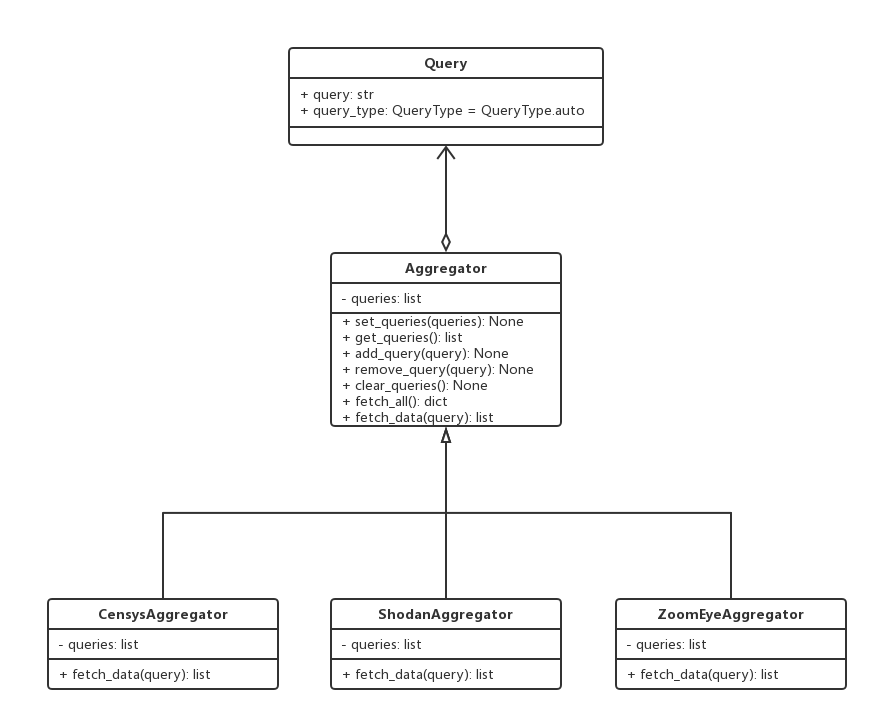
\includegraphics[scale=0.35]{hosts-aggregation-class.png}
    \caption{主机信息抓取模块类图}
    \label{fig:hosts-class}
\end{figure}

具体的Aggregator目前有3个,分别是CensysAggregator,ShodanAggregator和ZoomEyeAggregator。这三个类都继承了Aggregator类,
实现了其中的抽象方法。图~\ref{fig:hosts-class}是该模块的类图。从图中可以看出,三个具体的Aggregator类和Aggregator基类是继承关系,
而Aggregator和Query是聚合关系。

接下来依次介绍每一个API的信息抓取的类。

首先是CensysAggregator。Censys的API的参数中有一个是page,表示需要结果第几页,一页有100个结果,因此第一页就是第1至100个结果,
第二页就是第101至第200个结果,以此类推。因此在CensysAggregator内部又实现了一个方法fetch\_page,可以抓取一页最多100条结果的信息。
而在返回的结果中,有一个字段“metadata”会记录这些结果的元数据,在“metadata”字段中的“pages”字段就能知道这个关键词的搜索结果会有多少页。
所以,首先获得第一页的数据,看到有多少页之后循环获得后面几页的数据后再合并成一个新的列表,再给每个结果加上一个“source”字段赋值为“Censys”即可。

然后是ShodanAggregator。类似于Censys,Shodan的结果也是分页的,但是由于Shodan的API /search的结果只返回部分数据,
需要对每一个结果主机再次进行查询,因此,对每一个主机仅记录其IP地址,然后再对每一页的IP地址列表进行合并,删除重复的。
接着用另一个成员方法get\_info\_by\_ip获得其中每一台主机的详细信息,最后加入“source”字段赋值为“Shodan”。其中值得注意的一点是,
/host的API是有失败的可能的,因此在实现的时候设置了一个尝试次数,用try语句尝试几次,如果都失败了才最终返回一个只含IP地址的主机信息。

最后是ZoomEyeAggregator。ZoomEye的做法和Censys基本一样,也是先获得一页的内容然后再判断有多少页,
不过稍微不同的是ZoomEye没有直接提供页数的字段,而是总的可用的条目数“available”,需要自己计算页数。
在ZoomEyeAggregator中还实现了一个方法get\_latest,这个方法是在进行融合的时候使用。因为ZoomEye提供数据里面有重复的,
因此在融合的时候需要把相同主机的数据里面选出更新时间最近的数据,也即“timestamp”字段最大的数据。

\section{CVE信息抓取模块}
\label{sec:CVE-module}

CVE信息的抓取虽然也属于信息的抓取,但是和主机信息的抓取的方法和结构完全不一样,所以不需要继承Aggregator类,
而是定义了一个新的类CVEAggregator,专门用于CVE信息的抓取。

类似于Aggregator的设计,在CVEAggregator中也加入了一个私有变量cves,用于存放需要获取信息的CVE列表。在实际使用中,类似地,
先实例化一个对象,设定该列表之后调用update\_cves方法来更新列表中的CVE。而针对整个列表,也实现了一些相关的增删操作。

然而,在开始获取CVE信息前,大部分情况下是不知道CVE的名称的,如果想要获得所有的CVE信息,或者某几年的CVE信息,需要首先得到这些CVE的名字,
才能访问网页来进行爬虫的工作。因此,内部还实现了一个get\_all\_cves方法用于获得目前所有的CVE的名字的列表和一个get\_cves\_by\_years方法用于获得某几年的CVE的名字的列表。
其中后一个方法依赖于前一个方法,也即获得某几年的列表的时候,是首先获得全部的CVE列表再挑出来哪些是这几年的的。
而获得所有CVE的名字的列表的方法也是去访问一个链接,这个链接以纯文本的格式记录了所有的CVE的基本信息,可以用爬虫的方法获得其中的CVE名称。

而对于任意一个CVE,爬取其信息的方法就是标准的爬虫方法,先用CVE的名称得到对应的CVE的信息的页面,然后用requests库得到其HTML,
接着用BeautifulSoup解析该页面找到相应的数据即可。不过,有一些在前述方法中得到的CVE名称在CVE Details网站里不存在,需要提前判断排除。
此外,有的网站存在不规范的现象,比如内含非法字符“\&\#”,后面跟的内容不是数字无法构成字符,需要用正则表达式匹配去除该字符。

\section{数据库操作模块}
\label{sec:database-module}

在本系统中,有主机信息、CVE信息和威胁情报信息都需要进行存取的操作,其中主机信息是从API中获得的,在未经加工和融合之后的情况下是字典,
很容易格式化为json,而且内部存在非常复杂的字典和列表的嵌套关系;而CVE信息是系统抓取的,也存为字典;威胁情报也是系统分析的,在内存中存也为字典。
对于这种字典和列表有复杂嵌套关系的数据,非常容易选择数据库的类型为非关系型数据库,因此系统中选择的数据库为MongoDB\cite{chodorow2013mongodb},
而且Python中也有pymongo模块,可以轻松地操作MongoDB中的增删改查。

实现的时候,采用的方法是类似于namespace的方法定义个了一个MongoHelper类,实际上这个类并没有成员变量也没有成员方法,
都是静态方法,这么做的目的是不希望有数据库读写的方法散落在各个文件中,希望可以集中所有的数据库操作的方法到一起,也能方便修改和调试。

在本系统中,共有1个数据库和三个Collection,分别存储主机的信息、CVE的信息和分析结果的威胁情报信息。在该类中,
所有的方法都是围绕这三个Collection进行增删改查,比如存储一系列主机信息的方法、根据IP地址找到一台主机的信息的方法、
根据CVE名字获得威胁情报的方法等。存储的方法主要用于数据抓取的过程,而读取的方法主要用于网站的实现,在网站中,
为了给用户呈现尽量多的数据和用户体验,实现了很多根据某一些条件查询另一些数据的方法。

\section{推送模块}
\label{sec:notification-module}

推送服务是在一次抓取信息和分析威胁结束之后做的,由系统发送邮件给用户,通知本次分析的结果,比如共多少台主机存在可能的高危漏洞,
用户关注的CVE中各有多少台主机可能受到威胁等。

这里采用的发送邮件的方法是使用SMTP协议,用Python的smtplib模块。在一次扫描结束后,建立一个smtplib.SMTP对象,填写服务器地址和端口两个参数,
然后用格式化的数据编辑好通知内容,发送给用户的之前设定好的邮箱。但是,用这种方法很容易产生的一个问题就是会被放入垃圾邮件甚至直接删除,
这里就需要用户主动添加发件人的邮箱至白名单了。因为用SMTP发送邮件是最简单的做法,而正因为如此目前大部分邮箱服务都提供了过滤的功能,
避免过多垃圾邮件。

\section{中控模块}
\label{cha:controller-module}

\subsection{控制信息获取功能}
\label{sec:controller-aggregation}

中控模块是本系统最核心的一个模块,第~\ref{sec:process}节中的系统流程图中的所有步骤都是该模块所做,
而其所做工作中除了初始化外第一步就是控制各个Aggregator抓取网络中的主机和CVE的信息。

在中控类Controller中存有queries和cves两个成员变量,分别存储当前本系统需要获取主机的信息的Query列表和CVE列表。
在Controller的主要函数start\_aggregate中,首先初始化这两个变量,然后开始主机信息的抓取和CVE信息的抓取。

在主机信息的抓取中,首先初始化三个Aggregator的对象,然后设定它们各自的queries为Controller的queries,
接着就调用fetch\_all开始各自的抓取工作。在各自的工作都完成之后,就开始融合三个数据源的主机信息,使用的方法即第~\ref{sec:merge-strategy}节中介绍的方法。
不过,此处稍有不同的是,在最后一步存储数据进入数据库前,需要对融合的数据进行进一步的处理,因为MongoDB对存储的数据有要求。
比如MongoDB最大存储64位整数,而有一个“serial”字段的值可能会超过$10^{30}$,此时就需要把这个值转换成字符串再存入数据库。
又如MongoDB要求字典的键中不能含有“.”,而比如“metadata.os”这个键就含有,异或其他更加深层的键中也有。此处采用递归的方法对所有的键进行遍历,
把点换成了下划线。诸如此类的特殊处理是在实际操作中一个一个排查的,可能在API信息的扩充中需要增加新的特殊处理。

而在CVE信息的抓取中,同样是初始化一个CVEAggregator对象然后初始化抓取目标后进行抓取,但是为了提高效率,
此处采用了多线程的方法让同时有多个对象在进行信息的抓取。每个线程中都有一个抓取用的对象,然后在初始化的时候去访问共享变量cves,
取其中的前定值个CVE(目前设定为100),然后开始这些CVE的详情抓取。为了解决同步互斥的问题,在访问全部CVE列表前需要获得锁。
在一个线程完成自己的一小部分工作后,它还回去重新访问这个列表看看任务有没有被拿空,如果没有则继续拿若干个,空了则该线程结束工作。
因为抓取的CVE的之间各个都没有依赖关系,所以可以用这种方式提高效率。

\subsection{分析威胁情报功能}
\label{sec:controller-analysis}

在抓取完主机和CVE信息之后就需要进行分析威胁情报了。

在进行分析的时候采取的方法和第~\ref{sec:comparation-strategy}节中介绍的方法完全一致,只是为了提高效率同样采用了多线程的处理方法。
如果设主机的数量为$n$,CVE的数量为$m$,为了对每一台主机遍历全部的CVE,时间复杂度至少为$O(mn)$,这是一个非常长的时间,
而对每一台主机进行分析之间并没有依赖关系,所以可以采用多线程的方法节省时间。此处的方法同样类似CVE处理的时候的处理方法,
每个线程都在开始任务前取共享变量的主机列表中的若干项,然后处理完成后重新访问再去访问直到取空。

\subsection{配置文件}
\label{sec:controller-config}

在第~\ref{sec:controller-aggregation}节中提到Controller类中有两个成员变量queries和cves,为了设置这两个变量的值,
不是在代码中设置,而是使用配置文件config.json来设置这两个变量。在配置文件中,不仅能够设置需要监测的主机范围和CVE范围,
还能设置推送的时候推送的邮箱列表和着重关注的CVE列表。

在这个文件中,任何字段都有其固定的格式,比如“CVEs”这个字段里面的二级字段“years”可以设定CVE的年份,“others”可以添加一些其他的CVE,
“all”为True表示监测全部CVE。

在初始化的时候,由Controller来解析这个文件并填入这两个变量,之后的操作中都可以用成员变量来访问就不需要再访问文件了。

\subsection{定时功能}
\label{sec:controller-timer}

为了让系统具有实时性,并且各个API也是定时更新的,CVE Details和全部CVE的列表也是会更新的,定时更新整个数据库就变得很有必要。
此处定时采用的方法比较简单,即把Controller运行在另一个进程中,而非另一个线程(为了避免GIL的问题),
然后在Controller完成一次start\_aggregate之后,调用time.sleep,推迟线程的运行,在到达设定时间之后,Controller会再次运行。
目前设定的时间周期是一周,也即公式~\ref{equ:week}

\begin{equation}
    \label{equ:week}
    7 \times 24 \times 60 \times 60 = 604800 \, sec
\end{equation}

将该参数填入sleep的参数中即可。

在启动系统的时候,需要首先启动Controller,然后再启动服务器。

\subsection{中控模块类图}
\label{sec:controller-class}

\begin{figure}[H]
    \centering
    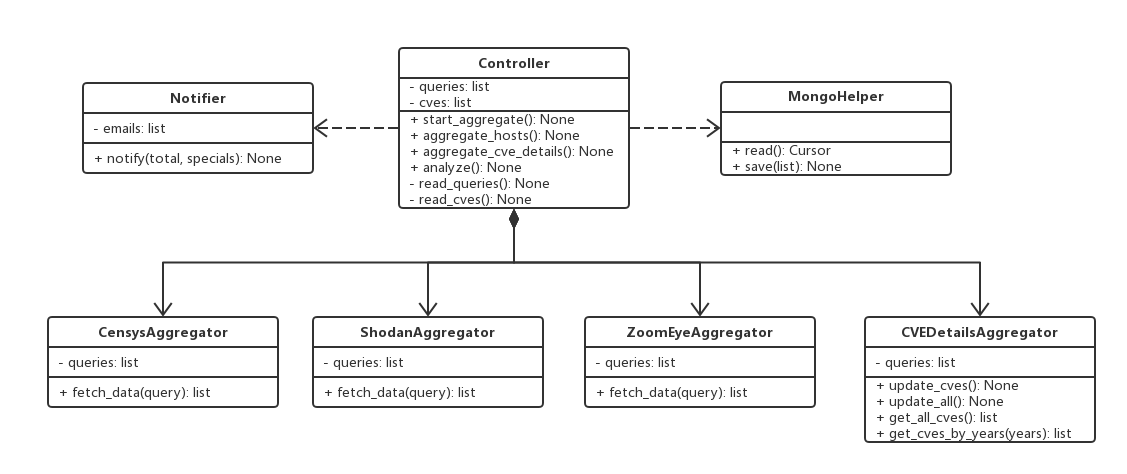
\includegraphics[scale=0.35]{controller-class.png}
    \caption{Controller的类图}
    \label{fig:controller-class}
\end{figure}

图~\ref{fig:controller-class}是Controller的类图。它描述了Controller类和之前描述的几个模块之前的关系,也即和各个Aggregator之间是组合关系,
而和Notifier和MongoHelper之间是依赖关系。

\section{网站}
\label{sec:website}

网站的模块是和主要逻辑无关的一个模块,为了让用户能更加简单地使用该系统,于是制作了一个简单的Flask框架的web网站。

网站总共分为/index展示有可能有高危漏洞的主机列表;/details展示某一台主机的详情,包括基本信息、高危CVE信息、开放端口和运行的服务等;
/search用来展示搜索的结果;/raw用来展示一台主机的json格式的详细信息的原始内容,共4个路径。

不论是哪个路径,基本的思路都是通过某些信息去查数据库,然后再通过jinja2模板引擎展示在页面上。
